\documentclass[10pt]{beamer}
\usepackage[utf8]{inputenc}
%\usepackage{xeCJK}
%\usetheme{Marburg}
\usetheme{Berkeley}


\setbeamerfont{note page}{size=\fontsize{0.2cm}{0.1cm}}

\usepackage{media9,tagging}
\usepackage{pgfplots}
\usepackage{amsmath}
\pgfplotsset{compat=1.10}
\usetikzlibrary{calc}
\usepackage[utf8]{inputenc}
\usepackage[T1]{fontenc}
\usepackage{comment}
\usepackage{mathtools}
\usepackage{bbold}
\usepackage{algorithmic}

\usepackage{xcolor}


%% Use any fonts you like.
\usepackage{helvet,multicol}
\newcommand\Newline{\newline\newline}

\DeclareUnicodeCharacter{2009}{\,} 


\usepackage{pstricks}


\title{\textcolor{white}{Algorithme Glouton faible par apprentissage}}
%\subtitle{\textcolor{white}{Subtitle}}
\author{Congo Job \\ 
sous la direction de Joubine Aghili }
\date{25 août 2022}
\institute{Université de Strasbourg\\Institut de Recherche de Mathématiques Avancées (IRMA)}


\begin{document}

\begin{frame}[plain,t]
\titlepage
\end{frame}


\section{Introduction}


\subsection{Contexte}

%--------- Contexte

\begin{frame}{Contexte}
\noindent%
\begin{minipage}{.6\textwidth}%
    \begin{itemize}
        \item 7 équipes de recherche
        \item 130 membres, dont 87 chercheurs et enseignants-chercheurs 
        \item Au sein de l'équipe "Modélisation et Contôle" 
    \end{itemize}
\end{minipage}%
\hfill
\begin{minipage}{.35\textwidth}%

\includegraphics[scale=0.12]{logo_irma.pdf}
\end{minipage}%
\end{frame}

\begin{comment}
Ce stage est réalisé à Institut de Recherche de Mathématiques Avancées (IRMA). L’IRMA est depuis 1997 une unité mixte de recherche
sous la double tutelle du CNRS et de l’Université de Strasbourg. Il fait partie de l’UFR de Mathématique et Informatique.
Elle compte quelques 130 membres, dont 87 chercheurs et enseignants-chercheurs permanents et une quarantaine de non-permanents répartis en 7 équipes de recherche. 
C'est avec l'équipe "Modélisation et contrôle" que le stage a eu lieu. 
Cette équipe s'intéresse à l’analyse des EDP, à l'optimisation, à la théorie du 
contrôle, au calcul scientifique et haute performance, et à la statistique. Ce stage a eu lieu du 1 juin 2022 au 31 juillet 2022.
\end{comment}


\subsection{Objectif du stage}


%---------------- Objectif 

\begin{frame}{Objectif}
Objectif : Trouver un substitut à l'erreur de projection dans l'algorithme glouton.

Dans le cadre des EDP paramétrée, la méthode des bases réduites  s'avère souvent être une option de premier choix.
\noindent%
\begin{minipage}{.65\textwidth}%
\begin{block}{Algorithme Glouton}
\begin{algorithm}
\begin{algorithmic}
\REQUIRE $\wedge_{test}$ un ensemble, $u_{EF}(\mu)$ et $u_{BR}(\mu)$ 2 fonctions
\STATE {choisir $\mu_1 $ de manière aléatoire}
\STATE {$u_1 = u_{EF}(\mu)$}
\STATE {$B_1 = Vect(u_1)$}
\FOR {$i$ allant de 2 à ${N_0}$ }
\STATE {$u_i := \underset{\mu \in \wedge_{test}}{argmax }(||u_{EF}(\mu) - P_{B_i}u_{BR}(\mu)||)$}
\STATE {$B_i := Vect(B_{i-1} \cup u_i)$}
\ENDFOR
\ENSURE retourner $B_{N_0}$ \\
\end{algorithmic}
\end{algorithm}
\end{block}
\end{minipage}%
\hfill
\begin{minipage}{.3\textwidth}%

Exemple d'EDP paramétrée :

$$
\begin{cases} 
 y'' + \mu y = 1  & \Omega   \\
u = 0  & \partial \Omega  \\
\mu  \text{ le paramètre  }
\end{cases}
$$

\end{minipage}%
\end{frame}




%---------------- Etapes du stage

\begin{frame}{Etapes du stage}
\noindent Objectif principal : Construire un algorithme Glouton faible avec une modèle entrainé par réseau de neurone. \\

\noindent Etapes du stage : 
        \begin{itemize}
            \item Implémenter un exemple en 1d en Python avec la méthode des éléments finis et donner une validation avec la solution exate.
            \item Implémenter la méthode des bases réduites et faire une validation.
            \item Entrainer un réseau de neurone apprenant l'erreur de projection à l'aide de PyTorch/TensorFlow.
            \item Extension au cas 2D avec Feel++ et les bibliothèques adaptées.
        \end{itemize}
\end{frame}





\section{Elements finis}

%--------------- Exemple 1D

\begin{frame}{Exemple 1D}

On s'intéresse au problème 1D paramétrée par $\mu$ issue d'un miniprojet d'Alexandre Ern \cite{Alexandre Ern}:
\begin{equation*}\label{moneq}
\begin{cases} 
- \frac{\partial }{\partial x}(D \cdot \frac{\partial u}{\partial x}) + u = f ,
 & \Omega   \\
u = 0  & \partial \Omega \\
D(x) = 
\begin{cases} 
1 , x \in \Omega _{1} \\
\mu , x \in \red \Omega _{2}
\end{cases}
\end{cases}
\end{equation*}

\begin{center}
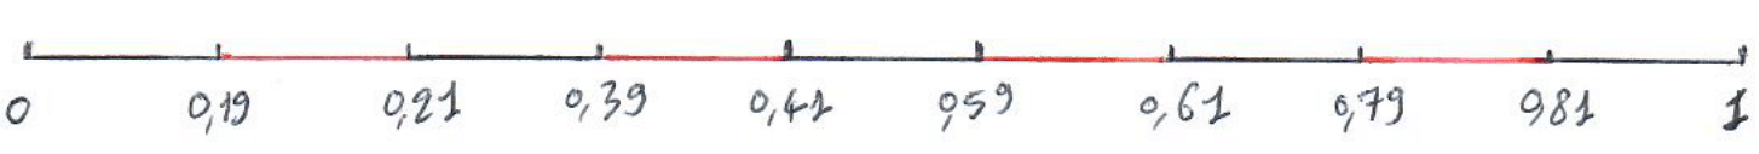
\includegraphics[scale = 0.35]{omega1.pdf}
\caption{Décomposition de $\Omega$ en $\Omega_1$ et $\Omega_2$}
\end{center}

\end{frame}

\subsection{Formulation Variationnelle}


%----------------- Formulation Variationnelle

\begin{frame}{Formulation Variationnelle}

La formulation variationnelle s'écrit: trouver 
$u \in H_{0}^{1}(\Omega)$ tel que :

\begin{equation*} 
a(u,v;\mu) = l(v) , \forall v \in H_{0}^{1}(\Omega)
\end{equation*}

En posant :
$$
\forall u, v \in H_{0}^{1}(\Omega) 
\hspace{0.5 cm}
a(u,v;\mu) := \int_{\Omega_{1}} v'u' + \mu\int_{\Omega_{2}}v'u' + \int_{\Omega} vu 
\text{, }
$$

$$
l(v) := \int_{\Omega} fv.
$$



\end{frame}





\subsection{Discrétisation du problème}



\subsubsection{Construction des espaces d’approximation }



%----------------- Discrétisation de $\Omega$

\begin{frame}{Discrétisation de $\Omega$}

Soit $\Omega $ un segment, que l'on décompose en $\Omega_{1}$ et 
$\Omega_{2}$ disjoints et construit un maillage équidistant : $$ \Omega = 
\bigcup_{i =0} ^{N - 1} K_i $$ 
tel que :
\begin{enumerate}
 \item $N$ est le nombre d'éléments du maillage et $h$ le pas constant vaut $ \frac{1}{N- 1}$.
 \item $ K_i = [x_i, x_{i+1}] $ avec $x_i$ les noeuds du maillage.
 \item On suppose que chaque maille $K_i$ se trouve soit dans $\overline{\Omega_1}$ soit dans $\overline{\Omega_2}$.
\end{enumerate}

\begin{center}
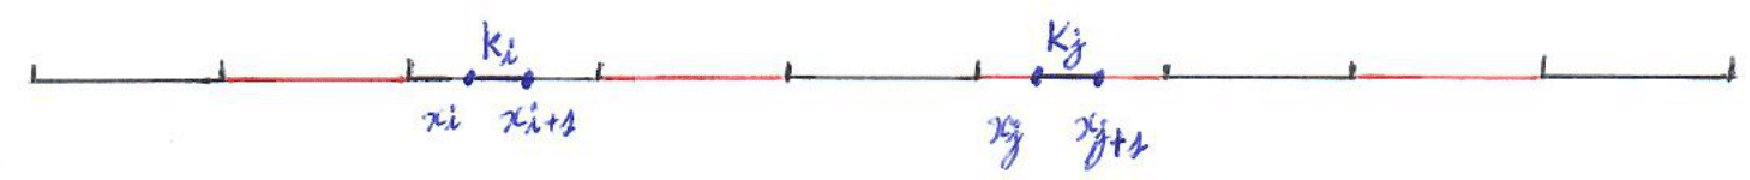
\includegraphics[scale = 0.35]{omega2.pdf}
\caption{Décomposition de $\Omega$ en $K_i$}
\end{center}
\end{frame}


%-----------------Discrétisation de $H^{1}_{0}(\Omega)$

\begin{frame}{Discrétisation de $H^{1}_{0}(\Omega)$}

\noindent Une discrétisation possible de $H^{1}_{0}(\Omega)$ est l’espace $V_{h,0}$ défini par : 
$$ 
V_{h,0} = \{u \in V_{h} \text{  }| \text{  } u_{| \partial \Omega} = 0 \} 
$$

$$ 
V_h  = Vect (\{\varphi_{i}\})  
$$

\begin{figure}
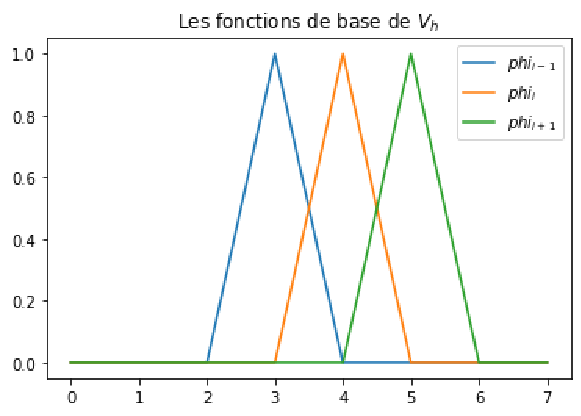
\includegraphics[scale=0.63]{fct_baseVh.pdf}
\end{figure}

\end{frame}



\subsubsection{Construction des matrices éléments finis}


%-----------------Problème approché

\begin{frame}{Problème approché}
\noindent En remplacant $H_{0}^{1}(\Omega)$ par $V_{h,0}$, on va chercher à résoudre le problème discret : 

\begin{equation*} 
\text{Trouver } u_h \in V_{h,0} \text{ tel que : } a(u_h, v_h;\mu) = l(v_h), \forall v_h \in V_{h,0}
\end{equation*}

\end{frame}


%-----------------Matrices éléments finis 1 correct


\begin{frame}{Matrices éléments finis}

\noindent Notons 
$$
A_{\mu} := 
\begin{pmatrix}
 &  &  & & \\
 &  &  &  & \\
 &  &  a(\varphi_{i},\varphi_{j};\mu)  &  & \\
  &  &  & & \\
 &  &  & &
\end{pmatrix} 
X :=\begin{pmatrix}
 \alpha_0   \\
 .  \\
 . \\
 . \\
\alpha_{N-1} 
\end{pmatrix} \text{ et } 
b := 
\begin{pmatrix}
\\
\\
l(\varphi_{j}) \\
\\
\\
\end{pmatrix}
$$

\noindent Résoudre le problème approché revient à touver $X_{\mu}$ tel que $$ A_{\mu}X_{\mu}=b$$
où :
\begin{enumerate}
    \item $A_{\mu} = A_{1} + \mu A_{2} + M $  
    \item $A_{1} = \int_{\Omega} \mathbb{1}_{\Omega_{1}} \varphi'_{i} \varphi'_{j}    \text{ ,  } A_{2} = \int_{\Omega} \mathbb{1}_{\Omega_{2}} \varphi'_{i} \varphi'_{j} \text{  ,  }  M = \int_{\Omega} \varphi_{i} \varphi_{j}$
    \item  $ b = \int_{\Omega} f \varphi_{j}$
\end{enumerate}

\end{frame}


%-----------------Matrices éléments finis 2 correct


\begin{frame}{Matrices éléments finis}

\noindent Posons 
$$
D := \begin{psmallmatrix}
2 & -1 & 0 &\dots & \dots &0   \\
-1 & 2 & -1 &0 & \dots &0   \\
 0 & -1 & 2 & -1 & 0 & 0    \\
\vdots  &  \ddots & \ddots  & \ddots & \ddots & \vdots \\
0  & \dots & 0  &-1 & 2 &-1 \\
0  &  \dots & \dots   &0 & -1 &2 
\end{psmallmatrix} 
$$


\noindent Après calculs on a :

\noindent%
\begin{minipage}{.35\textwidth}%

$$
A_{1} := \frac{1}{h}
\begin{psmallmatrix}
D & . & . & . & . & . & . & . & .\\
. & . & . & . & . & . & . & . & .\\
. & . & D & . & . & . & . & . & .\\
. & . & . & . & . & . & . & . & .\\
. & . & . & . & D & . & . & . & .\\
. & . & . & . & . & . & . & . & .\\
. & . & . & . & . & . & D & . & .\\
. & . & . & . & . & . & . & . & .\\
. & . & . & . & . & . & . & . & D
\end{psmallmatrix} 
$$
$$
A_{2} := \frac{1}{h}
\begin{psmallmatrix}
. & . & . & . & . & . & . & . & .\\
. & D & . & . & . & . & . & . & .\\
. & . & . & . & . & . & . & . & .\\
. & . & . & D & . & . & . & . & .\\
. & . & . & . & . & . & . & . & .\\
. & . & . & . & . & D & . & . & .\\
. & . & . & . & . & . & . & . & .\\
. & . & . & . & . & . & . & D & .\\
. & . & . & . & . & . & . & . & .
\end{psmallmatrix} 
$$
\end{minipage}%
\hfill
\begin{minipage}{.65\textwidth}%
$$
M:= h\begin{psmallmatrix}
\frac{2}{3} &  \frac{1}{6} & 0 &\dots & \dots &0   \\
\frac{1}{6} & \frac{2}{3} & \frac{1}{6} &0 & \dots &0   \\
 0 & \frac{1}{6} & \frac{2}{3} & \frac{1}{6} & 0 & 0    \\
\vdots  &  \ddots & \ddots  & \ddots & \ddots & \vdots \\
0  & \dots & 0  &\frac{1}{6} & \frac{2}{3} &\frac{1}{6} \\
0  &  \dots & \dots   &0 & \frac{1}{6} & \frac{2}{3}
\end{psmallmatrix} 
$$

$$
b := h
\begin{pmatrix}
0\\
1 \\
\vdots \\
1 \\
0
\end{pmatrix}
$$
\end{minipage}%



\end{frame}

%------------- poubelle
\begin{comment}

$$
(A_{1})_{ij} := \frac{1}{h}
\begin{pmatrix}
D & 0 & 0 & 0 & 0 & 0 & 0 & 0 & 0\\
0 & 0 & 0 & 0 & 0 & 0 & 0 & 0 & 0\\
0 & 0 & D & 0 & 0 & 0 & 0 & 0 & 0\\
0 & 0 & 0 & 0 & 0 & 0 & 0 & 0 & 0\\
0 & 0 & 0 & 0 & D & 0 & 0 & 0 & 0\\
0 & 0 & 0 & 0 & 0 & 0 & 0 & 0 & 0\\
0 & 0 & 0 & 0 & 0 & 0 & D & 0 & 0\\
0 & 0 & 0 & 0 & 0 & 0 & 0 & 0 & 0\\
0 & 0 & 0 & 0 & 0 & 0 & 0 & 0 & D\\
\end{pmatrix} 
$$
\end{comment}



%------------ poubelle
\begin{comment}

%-----------------Matrices éléments finis 

\begin{frame}{Matrices éléments finis}

Pour $\mu = 1$ et $Nel = 1000$, on a :

\noindent%
\begin{minipage}{.6\textwidth}%
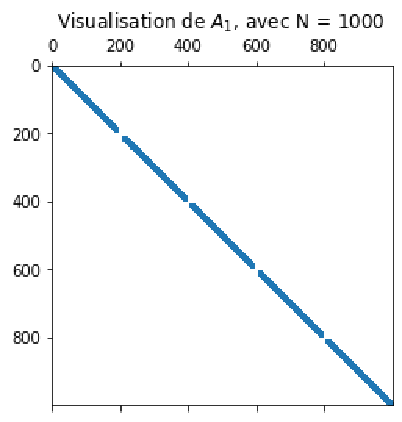
\includegraphics[scale=0.65]{visualA1.pdf}
\end{minipage}%
\begin{minipage}{.35\textwidth}%
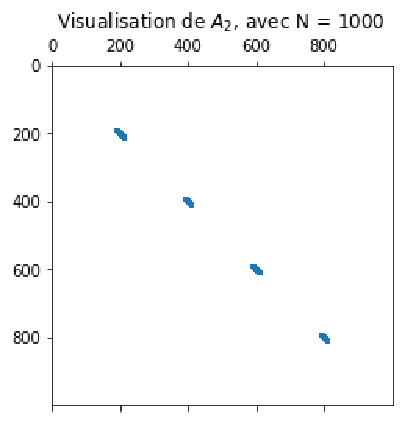
\includegraphics[scale=0.65]{visualA2.pdf}
\end{minipage}%
\end{frame}


\begin{frame}{Matrices éléments finis}


\begin{figure}
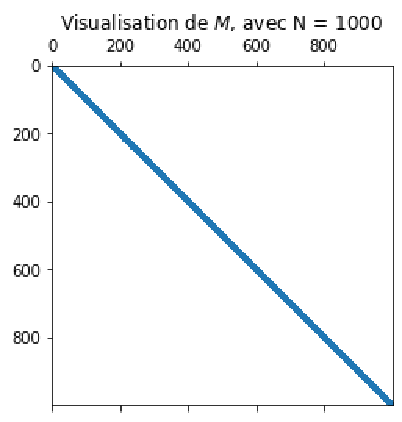
\includegraphics[scale=0.7]{visualM.pdf}
\end{figure}
\end{frame}


\end{comment}

\subsection{Validation}

%-----------------Validation
\begin{frame}{Validation}

Fixons $\mu = 1$ et le problème 1D se réécrit :
\begin{equation*}
\begin{cases}
-u'' + u = 1 \\
u|_{\partial \Omega} = 0
\end{cases}
\end{equation*}

Ce problème admet une unique solution $u_{ex}(x)$ connue:
$$
\forall x \in \Omega, u_{ex}(x) = C_{1}\exp(-x) + C_{2}\exp(x) +1 
$$
$$
\text{ avec }  C_{1} = \frac{1-e}{e - e^{-1}} \text{ et } C_{2} = \frac{e^{-1} - 1}{e - e^{-1}} 
$$

\end{frame}

\begin{comment}
On vérifie que si $\mu = 1 $ la solution éléments finis $u_{EF}$ est cohérente avec la solution exacte $u_{ex}$.
\end{comment}


%-----------------Estimations d'errreur
\begin{frame}{Estimations d'errreur}

%---- presenter les résultats en norme L2et H1

Quelques résultats pour évaluer la solution $u_{EF}$ : 

 $$ ||u-u_{h}||_{1,\Omega} \leq ch|u|_{2,\Omega} $$


 $$||u-u_{h}||_{0,\Omega} \leq ch^{2}|u|_{2,\Omega}$$

où $ u \in H^{2}(\Omega)$ et $c \geq 0 $ est indépendant de $h$

\end{frame}

\begin{comment}
On note $||.||_1$ la norme $H^{1}$, et $||.||_0$ la norme $L^{2}$
\end{comment}

%-----------------Illustration des Résultats
\begin{frame}{Illustration des Résultats}
Pour $N = 100$, on a :

\begin{center}
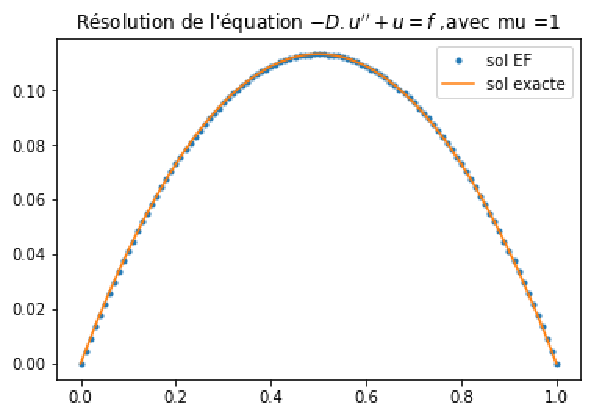
\includegraphics[scale=0.84]{sol_ef_exa.pdf}
\text{Solution exacte $u_{ex}$ et solution élément fini $u_{EF}$} 
\end{center}

\end{frame}

%-----------------Illustration des erreurs
\begin{frame}{Illustration des erreurs}
Pour diverses valeurs de $N $, on a:

\begin{center}
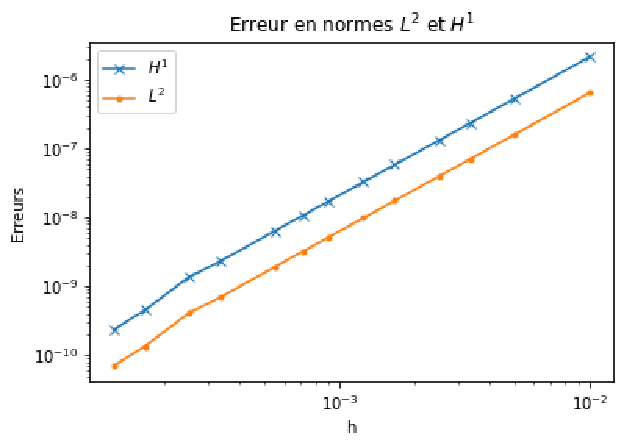
\includegraphics[scale=0.8]{erreurL2H1V2.pdf}
\text{Erreurs $|| u_{ex} - u_{EF}||_{L^{2}}$ et $|| u_{ex} - u_{EF}||_{H^{1}}$ en fonction de h}
\end{center}

\end{frame}


\begin{comment}
nous avons résolu le problème \eqref{eqnum1} et calculer l'erreur entre $u_{ex}$ et $u_{EF}$ en norme $H^1$ et $L^{2}$. La pente de l'erreur est de $2$ en norme $H^1$ et $L^{2}$, ce qui est conforme aux attentes théoriques.
   
\end{comment}








\section{Modèle réduit}


\subsection{ Formulation du problème réduit }


%-----------------Modèle réduit 1

\begin{frame}{Modèle réduit}

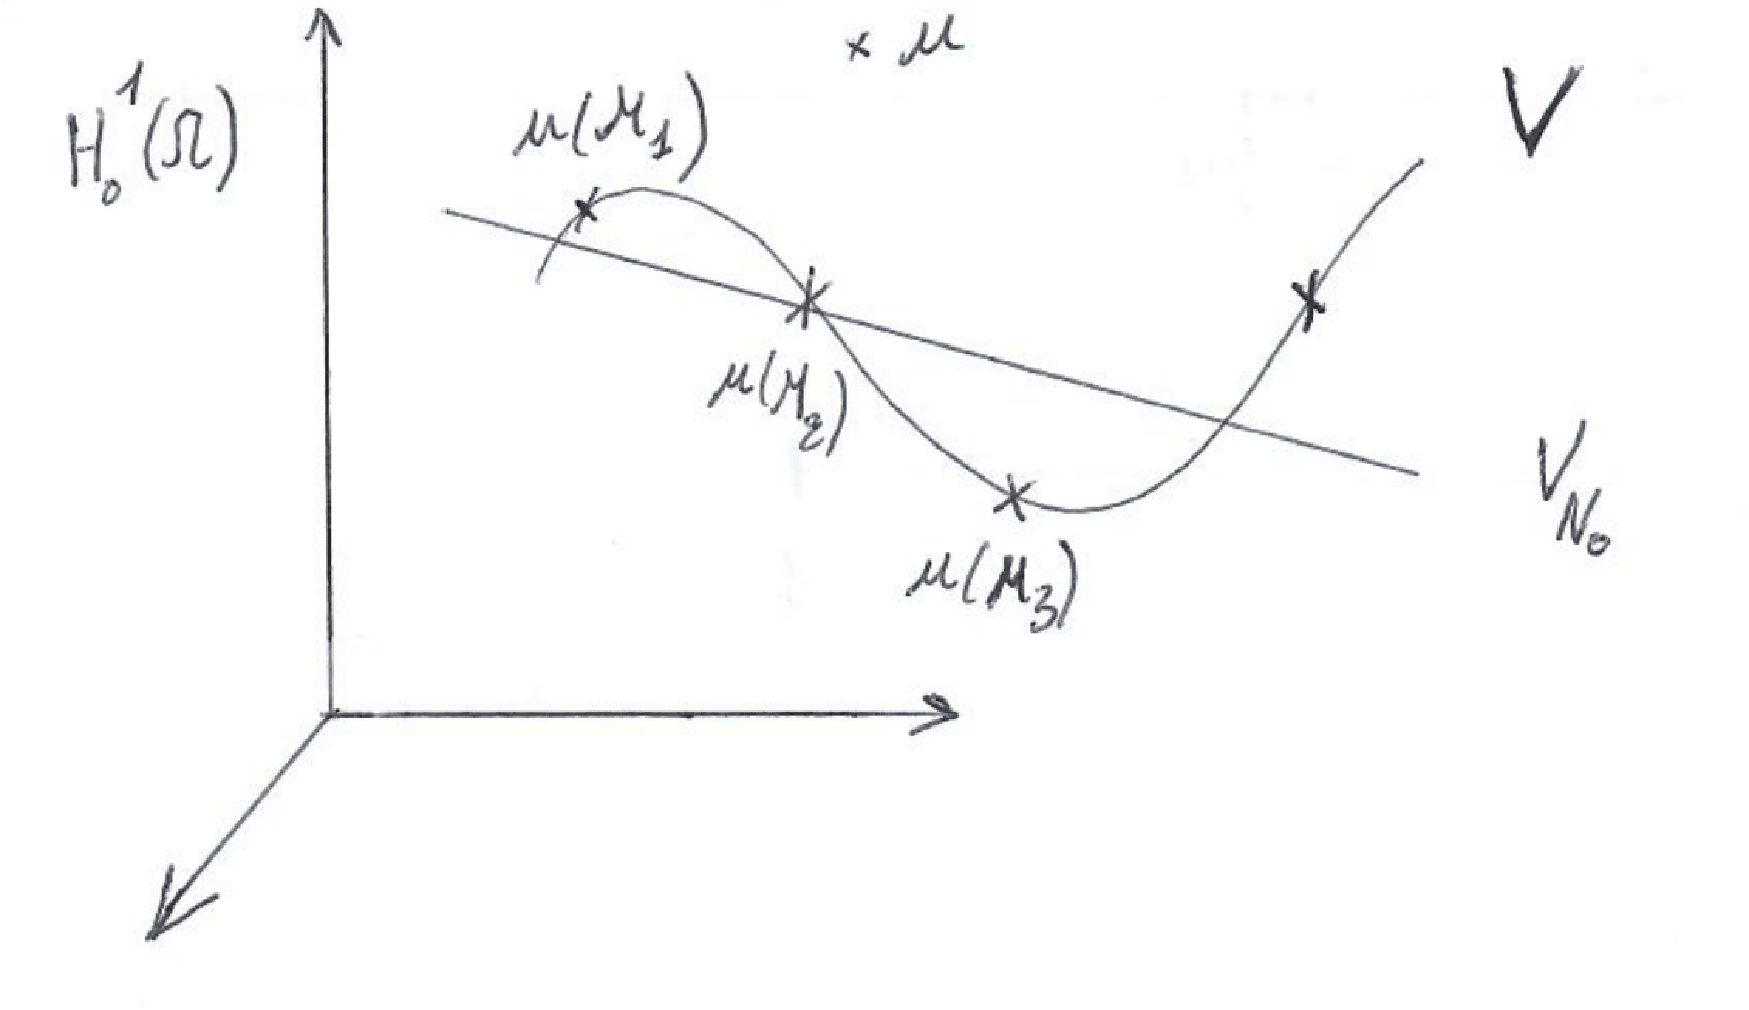
\includegraphics[scale = 0.3]{variete.pdf}

\noindent La méthode des bases réduites s’appuie sur le fait que les solutions de l’EDP vivent sur unevariété V.
On fait l'hypothèse fondamentale que $V \approx V_{N_{0}}$, avec $V_{N_{0}}$ un espace affine de faible dimension. 
 
\end{frame}

%-----------------Modèle réduit
\begin{frame}{Modèle réduit}


On cherche $
X^{br}_{\mu} :=
\begin{pmatrix}
x^{br}_{\mu,1}\\
\vdots \\ 
x^{br}__{\mu,N_{0}}
\end{pmatrix}
$
 tel que $$ u^{br}(\mu) = x^{br}_{\mu,1}u_1 + ... + x^{br}_{\mu,N_{0}}u_{N_{0}}$$

\noindent Les fonctions $u_i$ sont appelés «snapshot», et sont obtenues en résolvant le problème approché par éléments finis.
 
\end{frame}


\subsection{Espace des bases réduites $V_{N_{0}}$}


%-----------------Construction de la base réduite

\begin{frame}{Construction de la base réduite}
On définit  $ \wedge_{test} \subset \wedge = \mathbb{R_{*}^{+}}$

\noindent En pratique : 
$$\wedge_{test} := \{\mu_1,..., \mu_{M} \} \text{ et } M \approx 100$$ 

Grâce à l'algorithme Glouton avec $\wedge_{test}$, on a la base réduite  :

$$ V_{N_{0}} := vect(u_1,u_2,..., u_{N_0}) \text{ et } \wedge_{trial} := \{\mu_1,..., \mu_{N_{0}} \}$$



\end{frame}




\subsection{Matrices réduites}

%-----------------Matrices réduites 

\begin{frame}{Matrices réduites}
\noindent En posant
$$
U = \begin{pmatrix}
u_1, ..., u_{N_0}
\end{pmatrix} 
$$

\noindent Et construisant 
$$
V_{0}^{BR} := U^{T}(A_0 + M)U  \quad \text{   et   }  \quad  V_{1}^{BR} := U^{T}A_1U
$$

\noindent Avec les relations suivantes :
$$
B^{BR} := U^{T}b \text{    et    } A^{BR}_{\mu} = V_{0}^{BR} + \mu V_{1}^{BR}
$$

\noindent Résoudre le problème réduit  revient finalement à trouver $X^{br}_{\mu}$ tel que :
$$A^{BR}_{\mu} X^{br}_{\mu} = B^{br} $$ 




\end{frame}


\begin{comment}

\noindent À l’étape hors-ligne, le vecteur $B^{BR}$ et les matrices $V_{0}^{BR}$ et $V_{1}^{BR}$ sont calculées une seule fois. À l’étape en-ligne, pour un certain $\mu \in P_{trial}$, on assemble la matrice $A^{BR}_{\mu}$ et resout le système réduit $$A^{BR}_{\mu} X^{BR} = B^{BR}$$

\end{comment}



\subsection{Etude du modèle réduit}


\begin{comment}
Dans cette section, nous allons analyser la solution réduite du problème \eqref{eqnum1}. Pour ce faire, il faut d'abord choisir la valeur $N_{0}$ afin d'appliquer l'algorithme glouton.

Après la construction de $V_{0}^{BR}$ et $V_{1}^{BR}$ pour diverses valeurs de $N_{0}$, nous avons calculé leur conditionnement respectif. Quand $N_{0}$ est supérieur ou égale à 5, le problème devient mal conditionné et leurs conditionnements sont alors de l'ordre de $10^{16}$ d'après le graphique \eqref{fig:1}. Lorsque $N_{0}$ est égal à 2, le résultat est très insuffisant. Les valeurs convenables de $N_{0}$ sont donc 3,4,5. 
Dans la suite, nous fixons $N_{0}$ à 3 pour avoir un conditionnement pas trop élevé.

\end{comment}


%-----------------Résolution BR avec $N_0 = 2$

\begin{frame}{Résolution BR avec $N_0 = 2$}

\begin{figure}
\begin{center}
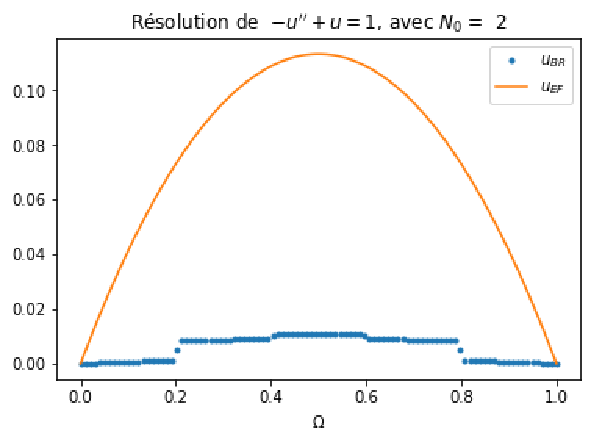
\includegraphics[scale=0.9]{sol_br_ef_2.pdf}
\text{Solutions Eléments Finis et Base Réduite }
\end{center}
\end{figure}

\end{frame}

%-----------------Résolution BR avec $N_0 = 3$

\begin{frame}{Résolution BR avec $N_0 = 3$}
\begin{figure}
\begin{center}
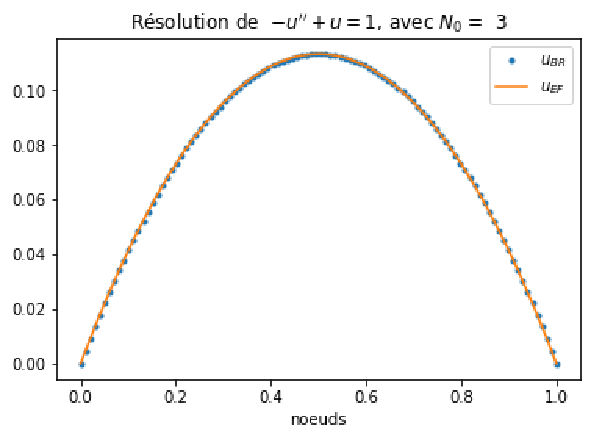
\includegraphics[scale=0.9]{sol_br_ef_3.pdf}
\text{Solutions Eléments Finis et Base Réduite }
\end{center}
\end{figure}

\end{frame}

%-----------------Résolution BR avec $N_0 = 4$

\begin{frame}{Résolution BR avec $N_0 = 4$}
\begin{figure}
\begin{center}
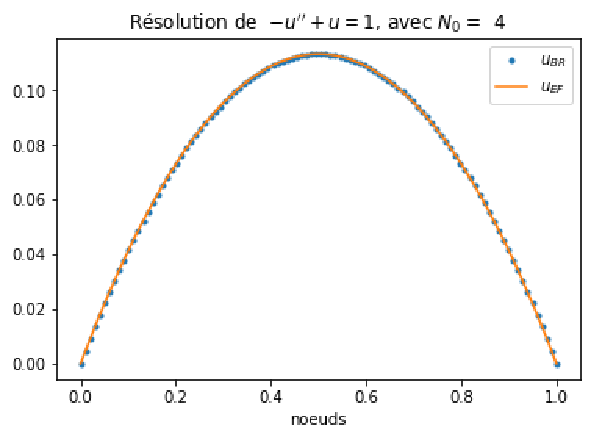
\includegraphics[scale=0.9]{sol_br_ef_4.pdf}
\text{Solutions Eléments Finis et Base Réduite }
\end{center}
\end{figure}

\end{frame}

%-----------------Résolution BR avec $N_0 = 5$

\begin{frame}{Résolution BR avec $N_0 = 5$}
\begin{figure}
\begin{center}
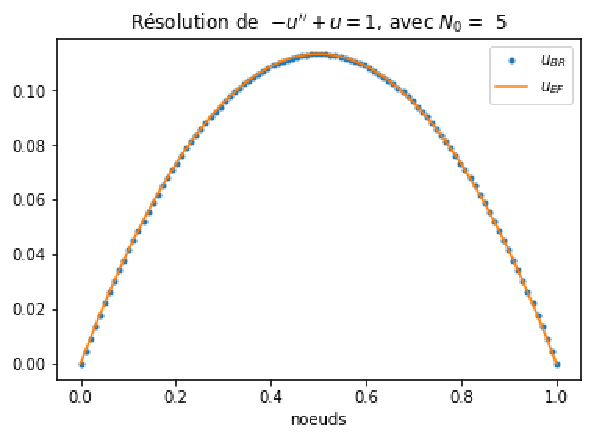
\includegraphics[scale=0.9]{sol_br_ef_5.pdf}
\text{Solutions Eléments Finis et Base Réduite }
\end{center}
\end{figure}

\end{frame}

%-----------------Le conditionnement

\begin{frame}{Le conditionnement}

\begin{figure}[H] 
\begin{center}
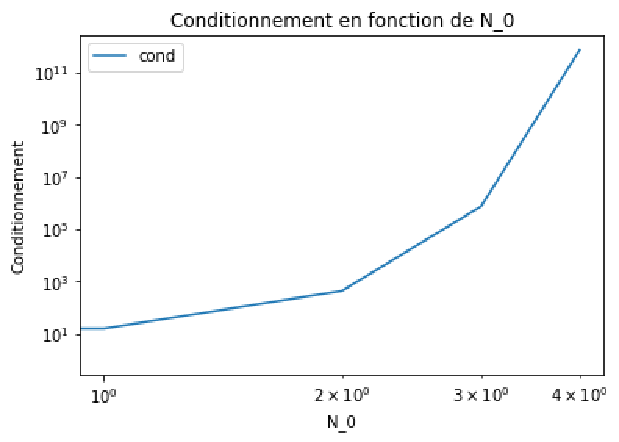
\includegraphics[scale=0.9]{cond.pdf}
\text{Evolution du conditionnement }
\end{center}
\end{figure}

\end{frame}

%-----------------Qualité de la base réduite
\begin{frame}{Qualité de la base réduite}

\noindent Après construction de $V_{N_{0}}$, on calcule  $$ \epsilon := \underset{\mu  \in  \wedge_{test}} {\sup}||u^{EF}(\mu) - u^{RB}(\mu) ||_{L^{2}} \text{ où }\wedge_{test} \cap \wedge_{trial} =  \emptyset $$

\begin{figure}
\begin{center}
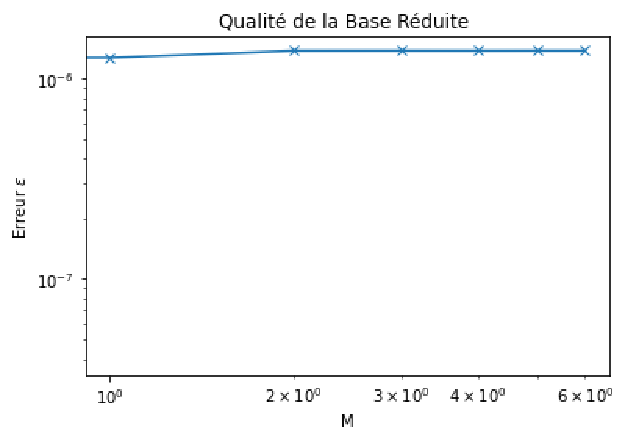
\includegraphics[scale=0.7]{qual_br.pdf}
\text{Erreur $\epsilon$ pour $M \in \{10,100,500,1000,2000,2500,3000\}$}
\end{center}
\end{figure}

\end{frame}


%-----------------Résolution avec $N_0 = 3$ et $\mu = 0.05$

\begin{frame}{Résolution avec $N_0 = 3$ et $\mu = 0.05$}
En fixant $\mu = 0.05$, voici la résolution du problème éléments finis et du problème réduit :

\begin{figure}
\begin{center}
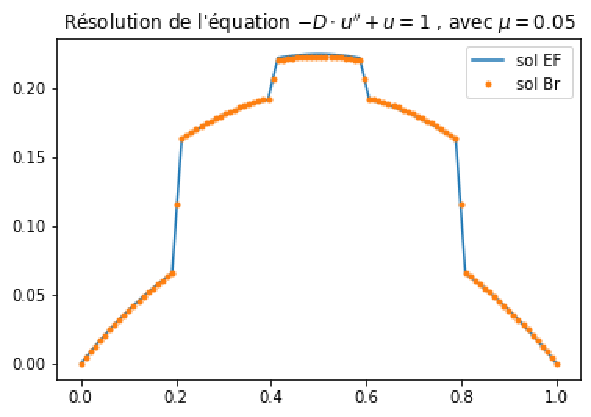
\includegraphics[scale=0.7]{sol_br_ef.pdf}
\text{Solution Elément Finis et Base Réduite pour $\mu = 0.05$ }
\end{center}
\end{figure}



\end{frame}

\begin{comment}
Comparons à présent la solution éléments finis avec celle du modèle base réduite. En fixant $\mu$ à 0.05, les résultats obtenus en utilisant la méthode des bases réduites et la méthode éléments finis sont cohérentes. En plus, l'erreur absolue entre les solutions éléments finis et base réduite inférieur à $10^{-3}$ \ref{fig:3}. 
\end{comment}


%----------------- Erreur absolue

\begin{frame}{Erreur absolue}

\begin{figure}
\begin{center}
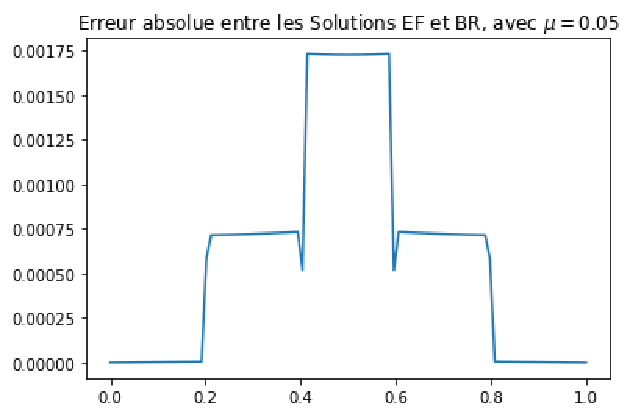
\includegraphics[scale=0.7]{err_br_ef.pdf}
\text{Erreur  en valeur absolu entre les solutions EF et BR pour $\mu = 0.05$ }
\end{center}
\end{figure}


\end{frame}


\section{Conclusion et perspectives}

%----------------- Conclusion et perspectives
\begin{frame}{Conclusion et perspectives}
Perspectives : remplacer $f(\mu) = \underset{\mu \in \wedge_{test}}{argmax }(||u_{EF}(\mu) - P_{B_i}u_{BR}(\mu)||)$  dans par un réseau de neuronne $NN(\mu)$ puis réaliser avec Feel++ l'extension 2D/3D. 

\begin{block}{Algorithme Glouton}
\begin{algorithm}
\begin{algorithmic}
\REQUIRE $\wedge_{test}$ un ensemble, $u_{EF}(\mu)$ et $u_{BR}(\mu)$ 2 fonctions
\STATE {choisir $\mu_1 $ de manière aléatoire}
\STATE {$u_1 = u_{EF}(\mu)$}
\STATE {$B_1 = Vect(u_1)$}
\FOR {$i$ allant de 2 à ${N_0}$ }
\STATE {$u_i := \underset{\mu \in \wedge_{test}}{argmax }(||u_{EF}(\mu) - P_{B_i}u_{BR}(\mu)||)$}
\STATE {$B_i := Vect(B_{i-1} \cup u_i)$}
\ENDFOR
\ENSURE retourner $B_{N_0}$ \\
\end{algorithmic}
\end{algorithm}
\end{block}

\end{frame}

\begin{comment}
LE solveur EF est pas cher en 1D , un peu cher en 2D et tres cher en 3D.
\end{comment}



\section{References}
\begin{frame}[allowframebreaks]{References}

\begin{thebibliography}{9}

\bibitem{Gianluigi Rozza}
Gianluigi Rozza,  \emph{An introduction to reduced basis method for parametrized PDEs
 }

\bibitem{B. Haasdonk}
B. Haasdonk,  \emph{Reduced Basis Methods for Parametrized PDEs –
A Tutorial Introduction for Stationary and
Instationary Problems }


\bibitem{Alexandre Ern}
Alexandre Ern,  \emph{ Analyse numérique et optimisation
Méthode des bases réduites }

\bibitem{Gwenol Grandperrin}
Gwenol Grandperrin,  \emph{Introduction à la méthode des bases réduites}

\end{thebibliography}
\end{frame}










%-----------------Matrices réduites 

\begin{frame}{Matrices réduites}
\noindent On sait que $u^{BR}_{\mu}$ et $u_i$  se décomposent sous la forme 
$$ 
u_{BR}^{\mu} = \sum_{i = 1}^{N_0} X^{BR}_{\mu, i}u_i 
$$
$$
u_i = \beta_0 \varphi_0 + ... + \beta_{Nel-1} \varphi_{Nel-1} 
$$

Et par billinéaire et linéarité de $l$ et $a_{\mu}$, on a :
$$
a_{\mu}(u^{BR}_{\mu}, u_i) = \sum_{i= 1}^{N_0}
\sum_{k, j= 0}^{Nel-1} X^{BR}_{\mu, i} 
\beta_{i, k} \beta_{i, j} a_\mu(\varphi_{k}, \varphi_{j})
$$
$$
l(u_i) = \sum_{i= 1}^{N_0}\sum_{j= 0}^{Nel-1} \beta_{i, j} l(\varphi_{j})
$$

\end{frame}

%-----------------Matrices réduites 

\begin{frame}{Matrices réduites}
\noindent Posons maintenant
$$
X^{br} = \begin{pmatrix}
X^{br}_{\mu,1} \\
. \\
. \\
. \\
X^{br}_{\mu,N_0} \\
\end{pmatrix} 
U = \begin{pmatrix}
u_1, ..., u_{N_0}
\end{pmatrix} 
$$

\noindent On réécrit  sous forme matricielle :
$$
(U^{T}A_{\mu}U)X^{br} = 
U^{T}(A_0 + M)U + \mu U^{T}A_1U = U^{T}b 
$$

\noindent Notons 
$$
V_{0}^{BR} := U^{T}(A_0 + M)U  \quad \text{   et   }  \quad  V_{1}^{BR} := U^{T}A_1U
$$

\noindent Ainsi on a les relations suivantes :
$$
B^{BR} := U^{T}b \text{    et    } A^{BR}_{\mu} = V_{0}^{BR} + \mu V_{1}^{BR}
$$

\end{frame}

%-----------------Matrices éléments finis


\begin{frame}{Matrices éléments finis}

Les conditions aux bords sont imposés fortement dans la matrice $A_1$ et $b$.
$$
(A_{\mu})_{ij} =
\begin{cases}
A_{ij}, \forall i, j \in \{1,..., Nel-2\} \\
1 \text{, lorsque } $(i, j) = (0,0)$ \text{  ou  } $(i, j) = (Nel-1,Nel-1)$ \\
0 \text{, sinon} 
\end{cases}
$$

$$
b_{j} =
\begin{cases}
h, \forall j \in \{1,..., Nel-2\} \\
0 \text{, sinon} 
\end{cases}
$$


\end{frame}


%-------- presentation 



\begin{comment}
Bonjour job à tous, je vais vous présenter mon stage qui s'intitule Algorithme Glouton par apprentissage , ce stage est réalisé à l'IRMA et supervisé par Monsieur Aghili Joubine .Il s'est déroulé du 1 juin au 31 juillet.
\end{comment}


%----------- objectif 

\begin{comment}
Dans le cadre des EDP paramétrée,
\end{comment}




\end{document}




